\documentclass{article}
\usepackage{amsmath, amsfonts, import}
\usepackage[breakable]{tcolorbox}
\usepackage{tikz}

\subimport*{./}{macro}
\setlength\parindent{0px}
\tcbset{
  answerbox/.style={
    colback=gray!10,       % light gray background
    colframe=black!40,     % dark gray border
    boxrule=0.4mm,
    arc=1mm,
    left=1mm,
    right=1mm,
    top=1mm,
    bottom=1mm,
    width=\textwidth,
    before skip=5pt,
    after skip=10pt,
  }
}

\begin{document}
\setcounter{aprob}{0}
\title{Homework \#1}
\author{
    \normalsize{CSE 446: Machine Learning}\\
    \normalsize{Professors Natasha Jaques}\\
    \normalsize{Due: \textbf{Wednesday, April 23, 2025, 11:59pm}}\\
    \normalsize{57 points}
}
\date{{}}
\maketitle
\section*{Short Answer and ``True or False'' Conceptual questions}
\begin{aprob}
    The answers to these questions should be answerable without referring to external materials.  Briefly justify your answers with a few words.
    \begin{enumerate}
        \item\points{2} In your own words, describe what bias and variance are? What is bias-variance tradeoff?
        \item \points{2} What \textbf{typically} happens to bias and variance when the model complexity increases/decreases?
        \item \points{1} True or False: A learning algorithm will always generalize better if we use fewer features to represent our data. 
        \item \points{2} True or False: Hyperparameters should be tuned on the test set. Explain your choice and detail a procedure for hyperparameter tuning.
        \item \points{1} True or False: The training error of a function on the training set provides an overestimate of the true error of that function.
    \end{enumerate}
    \subsubsection*{What to Submit:}
    \begin{itemize}
        \item \textbf{Parts a-e:} Brief (2-3 sentence) explanation
        \item \textbf{Parts c-e:} True or False
    \end{itemize}
    \begin{tcolorbox}[colback=lightgray!10!white, colframe=black, title=A1.a]
        \begin{enumerate}
            \item[i)] $\textbf{Bias} = \eta(x) - \mathbb{E}_D[\hat{f_D}(x)]$ \\
            Bias is the difference between the true function, \( \eta(x) \), and the expected prediction of our
            model, \( \mathbb{E}_D[\hat{f_D}(x)] \). This means that if our model, ($\hat{f}$), has high bias, then our model cannot describe our data; it is far off from the data.
            The more simple a model is, the higher its bias tends to be since it doesn’t fit the data as well and has a higher training error.
    
            \item[ii)] $\textbf{Variance} = \mathbb{E}_D\left[ \left( \hat{f_D}(x) - \mathbb{E}_D[\hat{f_D}(x)] \right)^2 \right]$ \\
            Variance is the amount by which our model’s prediction would vary if we trained it on a different dataset. High variance means
            our model is sensitive to training data and may fit noise/outliers. Variance tells us how much our estimate will change as the
            data changes. In other words, how much our predictions would change between different realizations of our model ($\hat{f}$).
            Variance measures inconsistency of a model across different training subsets.

            \item[iii)] \textbf{Bias-variance tradeoff} describes the tradeoff between bias and variance in reducing the learning error,
            which is equal to the $\text{bias}^2 + \text{variance}$. When choosing a model, you want to minimize both bias and variance
            as much as possible to reduce overall error by choosing a model that has enough expressive power to capture the underlying trends
            of the data but not enough to cause high variance.
        \end{enumerate}
    \end{tcolorbox}
    \begin{tcolorbox}[colback=lightgray!10!white, colframe=black, title=A1.b]
        When the model complexity increases the bias decreases because the model more
        closely matches the data. However the variance increases because the
        model starts to conform tightly to the idiosyncrasies of the training data. This
        means that the model becomes more sensitive to the specific training examples including outliers
        in the data. \\\\
        When the model complexity decreases the bias increases because the model no longer closely
        matches the data. However the variance tends to decrease when the model complexity decreases
        because the model has less expressive power and therefore does not change much if we add or
        remove a few data points. In other words the model becomes more stable across different training subsets.
    \end{tcolorbox}
    \begin{tcolorbox}[colback=lightgray!10!white, colframe=black, title=A1.c]
        False \\\\
        You could have few features that have little to no correlation with what you are trying to predict
        which would be worse off than having more features that are strongly correlated with what you are trying 
        to predict and would therefore result in the learning algorithm generalizing better. In other words using fewer features
        doesn't always lead to better generalization because if we reduce features by eliminating highly predictive ones while
        keeping irrelevant ones, generalization will worsen. Although feature reduction can help prevent overfitting, it can also
        increase bias if important information is lost. The optimal feature set balances relevance and complexity.
    \end{tcolorbox}
    \begin{tcolorbox}[colback=lightgray!10!white, colframe=black, title=A1.d]
        False \\\\
        Hyperparameters should NEVER be trained on the test set because that would contaminate
        our testing data. The test set should really only be used ONCE to test your model. Hyperparameters
        should instead be tuned using the validation set. \\
        
        A procedure for hyperparameter tuning involves using k-fold cross validation: 
        \begin{itemize}
            \item Divide the data into a training set and testing set.
            \item Randomly divide the training data into \(k\) equal-sized folds.
            \item For each set of hyperparameters being considered:
            \begin{itemize}
                \item Train \(k\) models, each time using \(k{-}1\) folds for training and the remaining fold for validation.
                \item Compute the average performance across all \(k\) validation folds.
            \end{itemize}
            \item Select the hyperparameters with the best average cross-validation performance.
            \item Retrain the model on the entire training set using the selected hyperparameters.
            \item Evaluate the model on the untouched test set.
        \end{itemize}
    \end{tcolorbox}
    \begin{tcolorbox}[colback=lightgray!10!white, colframe=black, title=A1.e]
        False \\\\
        The training error of a function on the training set typically \textbf{underestimates} the true error of that function.
        This is because the model is evaluated on the same data it was trained on, and may fit noise in the data leading to overfitting.
        The true error reflects how the model performs on unseen data and is generally higher than the training error. Hence, the 
        training error alone is an overly optimistic view of the model's performance.
        The true generalization error is equal to the following:
        \begin{align*}
            \text{True Generalization Error} = \text{Irreducible Error} + \text{Learning Error} \\
            = \text{Irreducible Error} + \text{Bias}^2 + \text{Variance}
        \end{align*}
        Training error only reflects a part of this, it is partially related to bias, but misses the impact of variance and irreducible noise on unseen data.
        \end{tcolorbox}
        
\end{aprob}


\section*{Maximum Likelihood Estimation (MLE)}

\begin{aprob}
    You're the Reign FC manager, and the team is five games into its 2021 season. The number of goals scored by the team in each game so far are given below:
    
    \[
      [2, 4, 6, 0, 1].
    \]
    Let's call these scores $x_1, \dots, x_5$. Based on your (assumed iid) data, you'd like to build a model to understand how many goals the Reign are likely to score in their next game. You decide to model the number of goals scored per game using a \emph{Poisson distribution}. Recall that the Poisson distribution with parameter $\lambda$ assigns every non-negative integer $x = 0, 1, 2, \dots$ a probability given by
    \[
      \mathrm{Poi}(x | \lambda) = e^{-\lambda} \frac{\lambda ^ x}{x!}.
    \]
    
    \begin{enumerate}
        \item \points{5} Derive an expression for the maximum-likelihood estimate of the parameter $\lambda$ governing the Poisson distribution in terms of goal counts for the first $n$ games: $x_1, \dots, x_n$. (Hint: remember that the log of the likelihood has the same maximizer as the likelihood function itself.)
        \item \points{2} Give a numerical estimate of $\lambda$ after the first five games. Given this $\lambda$, what is the probability that the Reign score $6$ goals in their next game?
        \item \points{2} Suppose the Reign score 8 goals in their 6th game. Give an updated numerical estimate of $\lambda$ after six games and compute the probability that the Reign score $6$ goals in their 7th game.
    \end{enumerate}
    \subsubsection*{What to Submit:}
    \begin{itemize}
        \item \textbf{Part a:} An expression for the MLE of $\lambda$ after $n$ games and relevant derivation
        \item \textbf{Parts b-c:} A numerical estimate for $\lambda$ and the probability that the Reign score 6 next game.
    \end{itemize}
        \begin{tcolorbox}[colback=lightgray!10!white, colframe=black, title=A2.a]
            
            Let $x_1, x_2, \dots, x_n$ be the number of goals scored in the first $n$ games. We assume these are i.i.d.\ samples from a Poisson distribution with parameter $\lambda$. The probability mass function of a Poisson distribution is:
            \[
            \text{Poi}(x_i | \lambda) = \frac{e^{-\lambda} \lambda^{x_i}}{x_i!}
            \]
            Solve for the MLE $\hat{\lambda}$ such that:
            \[
\hat{\lambda} = \arg\max_{\lambda} \mathcal{L}(x_1, \dots, x_n \mid \lambda)
\]

            
            The likelihood function of the data is:
            \[
            L(x_1, \dots, x_n | \lambda) = \prod_{i=1}^{n} \frac{e^{-\lambda} \lambda^{x_i}}{x_i!}
            \quad \text{likelihood function of scoring } x_1, \dots, x_n \text{ in the first } n \text{ games}
            \]
            
            Take the log of the likelihood:
            \[
            \log L(x_1, \dots, x_n | \lambda) = \log \left( \prod_{i=1}^{n} \frac{e^{-\lambda} \lambda^{x_i}}{x_i!} \right)
            = \sum_{i=1}^{n} \log \left( \frac{e^{-\lambda} \lambda^{x_i}}{x_i!} \right)
            \]
            \[
            = \sum_{i=1}^{n} \left( \log(e^{-\lambda}) + \log(\lambda^{x_i}) - \log(x_i!) \right)
            = \sum_{i=1}^{n} \left( -\lambda + x_i \log \lambda - \log(x_i!) \right)
            \]
            
            To find the MLE, take the derivative with respect to $\lambda$:
            \[
            \frac{d}{d\lambda} \left( \sum_{i=1}^{n} \left( -\lambda + x_i \log \lambda - \log(x_i!) \right) \right)
            = \sum_{i=1}^{n} \left( \frac{d}{d\lambda} (-\lambda) + \frac{d}{d\lambda}(x_i \log \lambda) - \frac{d}{d\lambda}(\log(x_i!)) \right)
            \]
            \[
            = \sum_{i=1}^{n} \left( -1 + \frac{x_i}{\lambda} \right)
            = \sum_{i=1}^{n} \left( \frac{x_i}{\lambda} - 1 \right)
            \]
            
            Set derivative equal to 0:
            \[
            \sum_{i=1}^{n} \left( \frac{x_i}{\lambda} - 1 \right) = 0
            \Rightarrow \sum_{i=1}^{n} \frac{x_i}{\lambda} = \sum_{i=1}^{n} 1 = n
            \Rightarrow \frac{1}{\lambda} \sum_{i=1}^{n} x_i = n
            \Rightarrow \sum_{i=1}^{n} x_i = n\lambda
            \Rightarrow \hat{\lambda} = \frac{1}{n} \sum_{i=1}^{n} x_i
            \]
            
            The maximum likelihood estimate (MLE) of $\lambda$ is the average goal score:
            \[
            \boxed{\hat{\lambda} = \frac{1}{n} \sum_{i=1}^{n} x_i}
            \]
            \end{tcolorbox}
            
            \begin{tcolorbox}[colback=lightgray!10!white, colframe=black, title=A2.b]
                After the first five games, the goal counts are: $[2, 4, 0, 6, 1]$.
                
                We estimate the MLE of $\lambda$ as:
                \[
                \hat{\lambda} = \frac{2 + 4 + 0 + 6 + 1}{5} = \frac{13}{5} = 2.6
                \]
                
                Now compute the probability of scoring 6 goals in the next game:
                \[
                \mathbb{P}(6 \mid \lambda = 2.6) = \frac{e^{-2.6} \cdot 2.6^6}{6!}
                \approx e^{-2.6} \cdot \frac{308.915776}{720} \approx 0.032
                \]
                
                \[
                \boxed{\mathbb{P}(X = 6 \mid \lambda = 2.6) \approx 3.2\%}
                \]
                \end{tcolorbox}
                
                \begin{tcolorbox}[colback=lightgray!10!white, colframe=black, title=A2.c]
                    Suppose the team scores 8 goals in the 6th game. The updated goal counts are $[2, 4, 0, 6, 1, 8]$.
                    
                    We update our estimate of $\lambda$:
                    \[
                    \hat{\lambda} = \frac{2 + 4 + 0 + 6 + 1 + 8}{6} = \frac{21}{6} = 3.5
                    \]
                    
                    Now compute the probability of scoring 6 goals in the 7th game:
                    \[
                    \mathbb{P}(6 \mid \lambda = 3.5) = \frac{e^{-3.5} \cdot 3.5^6}{6!}
                    \approx e^{-3.5} \cdot \frac{1838.265625}{720} \approx 0.077
                    \]
                    
                    \[
                    \boxed{\mathbb{P}(X = 6 \mid \lambda = 3.5) \approx 7.7\%}
                    \]
                    \end{tcolorbox}
                    
\end{aprob}



\newpage
\section*{Polynomial Regression}
{\bf Relevant Files}\footnote{{\bf Bold text} indicates files or functions that you will need to complete; you should not need to modify any of the other files.}
\vspace{-1.2em}
\begin{multicols}{2}
    \begin{itemize}[noitemsep,nolistsep]
        \item \texttt{\bf polyreg.py}
        \item \texttt{linreg\_closedform.py}
        \item \texttt{plot\_polyreg\_univariate.py}
        \item \texttt{plot\_polyreg\_learningCurve.py}
    \end{itemize}
\end{multicols}

\begin{aprob}
    \points{10} Recall that polynomial regression learns a function $h_{\bm{\theta}}(x) = \theta_0 + \theta_1 x + \theta_2 x^2 + \ldots + \theta_d x^d$, where $d$ represents the polynomial's highest degree.  We can equivalently write this in the form of a  linear model with $d$ features
    \begin{equation}
        h_{\bm{\theta}}(x) = \theta_0 + \theta_1 \phi_1(x)  + \theta_2 \phi_2(x)  + \ldots + \theta_d \phi_d(x)  \enspace ,
    \end{equation}
    using the basis expansion that $\phi_j(x) = x^j$.  Notice that, with this basis expansion, we obtain a linear model where the features are various powers of the single univariate $x$.  We're still solving a linear regression problem, but are fitting a polynomial function of the input.\\
    
    Implement regularized polynomial regression in \texttt{polyreg.py}.  You may implement it however you like, using gradient descent or a closed-form solution.  However, I would recommend the closed-form solution since the data sets are small; for this reason, we've included an example closed-form implementation of linear regression in \texttt{linreg\_closedform.py} (you are welcome to build upon this implementation, but make CERTAIN you understand it, since you'll need to change several lines of it).  You are also welcome to build upon your implementation from the previous assignment, but you must follow the API below.  Note that all matrices are actually 2D numpy arrays in the implementation.\\
    
    \begin{itemize}[noitemsep, nolistsep]
        \item \texttt{\_\_init\_\_(degree=1, regLambda=1E-8)} : constructor with arguments of $d$ and $\lambda$
        \item \texttt{fit(X,Y)}: method to train the polynomial regression model
        \item \texttt{predict(X)}: method to use the trained polynomial regression model for prediction
        \item \texttt{polyfeatures(X, degree)}: expands the given $n \times 1$ matrix $X$ into an $n \times d$ matrix of polynomial features of degree $d$.  Note that the returned matrix will not include the zero-th power.\\
    \end{itemize}
    
    Note that the \texttt{polyfeatures(X, degree)} function maps the original univariate data into its higher order powers.  Specifically, $X$ will be an $n \times 1$ matrix $(X \in \mathbb{R}^{n \times 1})$ and this function will return the polynomial expansion of this data, a $n \times d$ matrix.  Note that this function will {\bf not} add in the zero-th order feature (i.e., $x_0 = 1$).  You should add the $x_0$ feature separately, outside of this function, before training the model.

    \begin{wrapfigure}{R}{0.42\textwidth}
        \centering
        \vspace{-1em}
        % \includegraphics[width=0.4\textwidth]{../img/polyregDegree8.png}
        \vspace{-1em}
        \caption{Fit of polynomial regression with $\lambda = 0$ and $d = 8$}\label{fig:polyregUnivariate}
        \vspace{-2em}
    \end{wrapfigure}

    By not including the $x_0$ column in the matrix \texttt{polyfeatures()}, this allows the \texttt{polyfeatures} function to be more general, so it could be applied to multi-variate data as well. (If it did add the $x_0$ feature, we'd end up with multiple columns of 1's for multivariate data.)\\
    
    Also, notice that the resulting features will be badly scaled if we use them in raw form.  For example, with a polynomial of degree $d = 8$ and $x = 20$, the basis expansion yields $x^1 = 20$ while $x^8 = 2.56 \times 10^{10}$ -- an
    absolutely huge difference in range.  Consequently, we will need to standardize the data before solving linear regression.  Standardize the data in \texttt{fit()} after you perform the polynomial feature expansion.  You'll need to apply the same standardization transformation in \texttt{predict()} before you apply it to new data.\\
    
    Run \texttt{plot\_polyreg\_univariate.py} to test your implementation, which will plot the learned function.  In this case, the script fits a polynomial of degree $d=8$ with no regularization $\lambda = 0$.  From the plot, we see that the function fits the data well, but will not generalize well to new data points.  Try increasing the amount of regularization, and in 1-2 sentences, describe the resulting effect on the function (you may also provide an additional plot to support your analysis).
    
    \subsubsection*{What to Submit:}
    \begin{itemize}
        \item 1-2 sentence description of the effect of increasing regularization.
        \item Plots before and after increase in regularization.
        \item \textbf{Code} on Gradescope through coding submission
    \end{itemize}
    \begin{tcolorbox}[colback=lightgray!10!white, colframe=black, title=A3]
        Increasing regularization penalizes large weights, encouraging the model to keep them
        smaller. This simplifies the model, reducing overfitting. But too much regularization
        can lead to underfitting. \\
        \vspace{0.5em}
        \begin{center}
        \begin{minipage}{0.45\textwidth}
            \centering
            \textbf{$\lambda = 0$} \\[0.3em]
            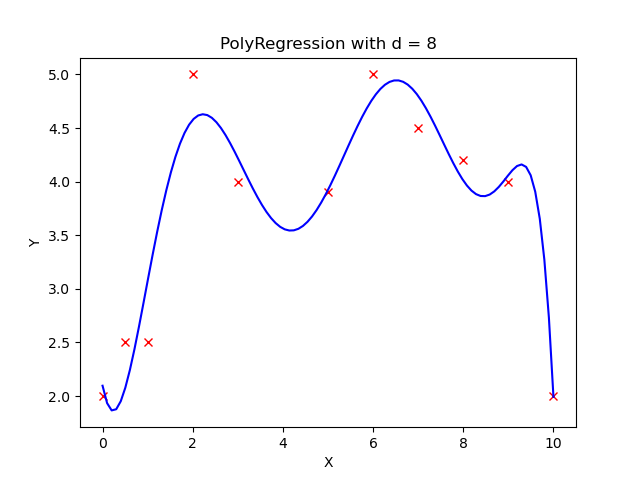
\includegraphics[width=\textwidth]{PolyRegression0Regularization.png}
        \end{minipage}
        \hfill
        \begin{minipage}{0.45\textwidth}
            \centering
            \textbf{$\lambda = 0.1$} \\[0.3em]
            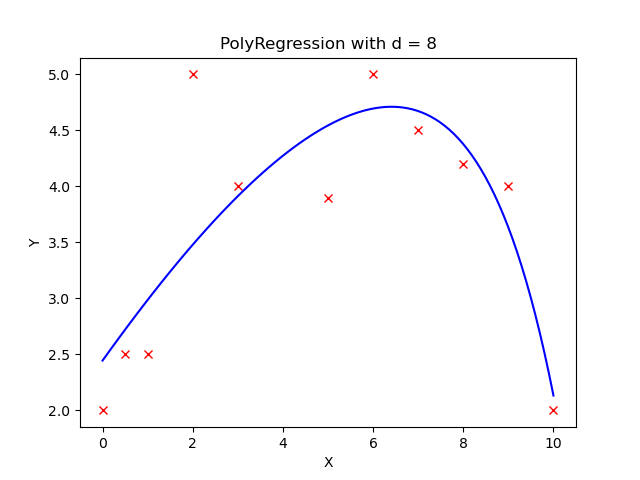
\includegraphics[width=\textwidth]{PolyRegression0.1Regularization.png}
        \end{minipage}
        
        \vspace{1em}
        
        \begin{minipage}{0.45\textwidth}
            \centering
            \textbf{$\lambda = 1$} \\[0.3em]
            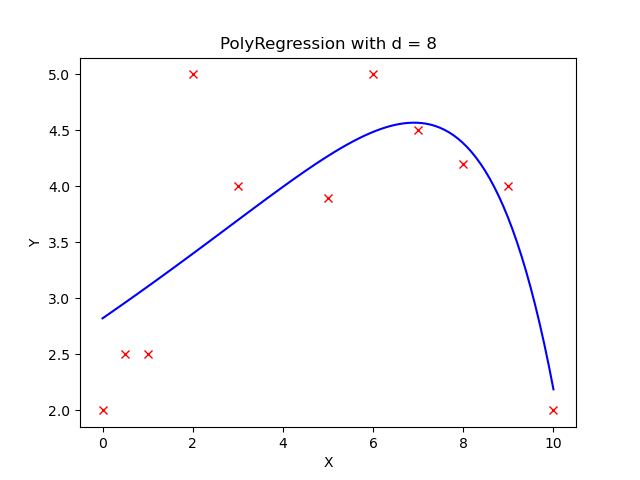
\includegraphics[width=\textwidth]{PolyRegression1Regularization.png}
        \end{minipage}
        \hfill
        \begin{minipage}{0.45\textwidth}
            \centering
            \textbf{$\lambda = 5$} \\[0.3em]
            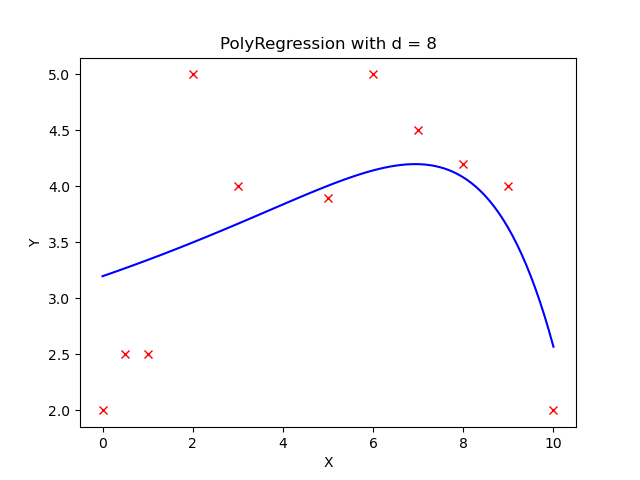
\includegraphics[width=\textwidth]{PolyRegression5Regularization.png}
        \end{minipage}
        
        \vspace{1em}
        
        \begin{minipage}{0.45\textwidth}
            \centering
            \textbf{$\lambda = 10$} \\[0.3em]
            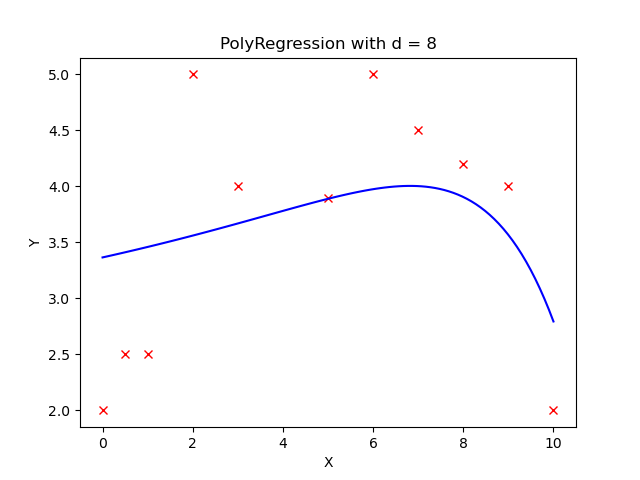
\includegraphics[width=\textwidth]{PolyRegression10Regularization.png}
        \end{minipage}
        \hfill
        \begin{minipage}{0.45\textwidth}
            \centering
            \textbf{$\lambda = 100$} \\[0.3em]
            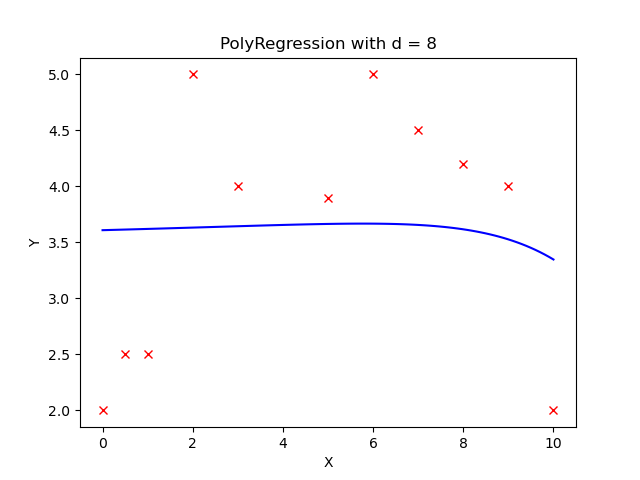
\includegraphics[width=\textwidth]{PolyRegression100Regularization.png}
        \end{minipage}
        \end{center}
    \end{tcolorbox}
\end{aprob}

\begin{aprob}
    \points{10} In this problem we will examine the bias-variance tradeoff through learning curves. Learning curves provide a valuable mechanism for evaluating the bias-variance tradeoff. Implement the \texttt{learningCurve()} function in \texttt{polyreg.py} to compute the learning curves for a given training/test set.  The \texttt{learningCurve(Xtrain, ytrain, Xtest, ytest, degree, regLambda)} function should take in the training data (\texttt{Xtrain}, \texttt{ytrain}), the testing data (\texttt{Xtest}, \texttt{ytest}), and values for the polynomial degree $d$ and regularization parameter $\lambda$. The function should return two arrays, \texttt{errorTrain} (the array of training errors) and \texttt{errorTest} (the array of testing errors).  The $i^{th}$ index (start from 0) of each array should return the training error (or testing error) for learning with $i +1$ training instances.  Note that the 0$^{th}$ index actually won't matter, since we typically start displaying the learning curves with two or more instances.\\
    
    When computing the learning curves, you should learn on \texttt{Xtrain}[0:$i$] for $i = 1, \ldots, \text{numInstances}(\texttt{Xtrain})$, each time computing the testing error over the {\bf entire} test set.  There is no need to shuffle the training data, or to average the error over multiple trials -- just produce the learning curves for the given training/testing sets with the instances in their given order.  Recall that the error for regression problems is given by
    \begin{equation}
        \frac{1}{n} \sum_{i=1}^n (h_{\bm{\theta}}(\mathbf{x}_i) - y_i)^2 \enspace.
    \end{equation}
    
    Once the function is written to compute the learning curves, run the \texttt{plot\_polyreg\_learningCurve.py} script to plot the learning curves for various values of $\lambda$ and $d$.  You should see plots similar to the following:
    \begin{figure}[ht!]
        \centering
        \vspace{-1em}
        % \includegraphics[width=\textwidth]{../img/polyregLearningCurves.png}
        \vspace{-1em}
    \end{figure}
    
    Notice the following:
    \begin{itemize}
        \item The y-axis is using a log-scale and the ranges of the y-scale are all different for the plots.  The dashed black line indicates the $y=1$ line as a point of reference between the plots.
        \item The plot of the unregularized model with $d = 1$ shows poor training error, indicating a high bias (i.e., it is a standard univariate linear regression fit).
        \item The plot of the (almost) unregularized model ($\lambda = 10^{-6}$) with $d = 8$ shows that the training error is low, but that the testing error is high.  There is a huge gap between the training and testing errors caused by the model overfitting the training data, indicating a high variance problem.
        \item As the regularization parameter increases (e.g., $\lambda = 1$) with $d = 8$, we see that the gap between the training and testing error narrows, with both the training and testing errors converging to a low value.  We can see that the model fits the data well and generalizes well, and therefore does not have either a high bias or a high variance problem.  Effectively, it has a good tradeoff between bias and variance.
        \item Once the regularization parameter is too high ($\lambda = 100$), we see that the training and testing errors are once again high, indicating a poor fit.  Effectively, there is too much regularization, resulting in high bias.
    \end{itemize}
    
    Submit plots for the same values of $d$ and $\lambda$ shown here. Make absolutely certain that you understand these observations, and how they relate to the learning curve plots.  In practice, we can choose the value for $\lambda$ via cross-validation to achieve the best bias-variance tradeoff.
    
    \subsubsection*{What to Submit:}
    \begin{itemize}
        \item \textbf{Plots} (or single plot with many subplots) of learning curves for $(d, \lambda) \in {(1, 0), (4,10^{-6}), (8, 10^{-6}), (8, 0.1), (8, 1), (8, 100)}$.
        \item \textbf{Code} on Gradescope through coding submission
    \end{itemize}
    \begin{tcolorbox}[colback=lightgray!10!white, colframe=black, title=A4]
        \begin{center}
            Learning curves for $(d, \lambda) \in {(1, 0), (4,10^{-6}), (8, 10^{-6}), (8, 0.1), (8, 1), (8, 100)}$.
            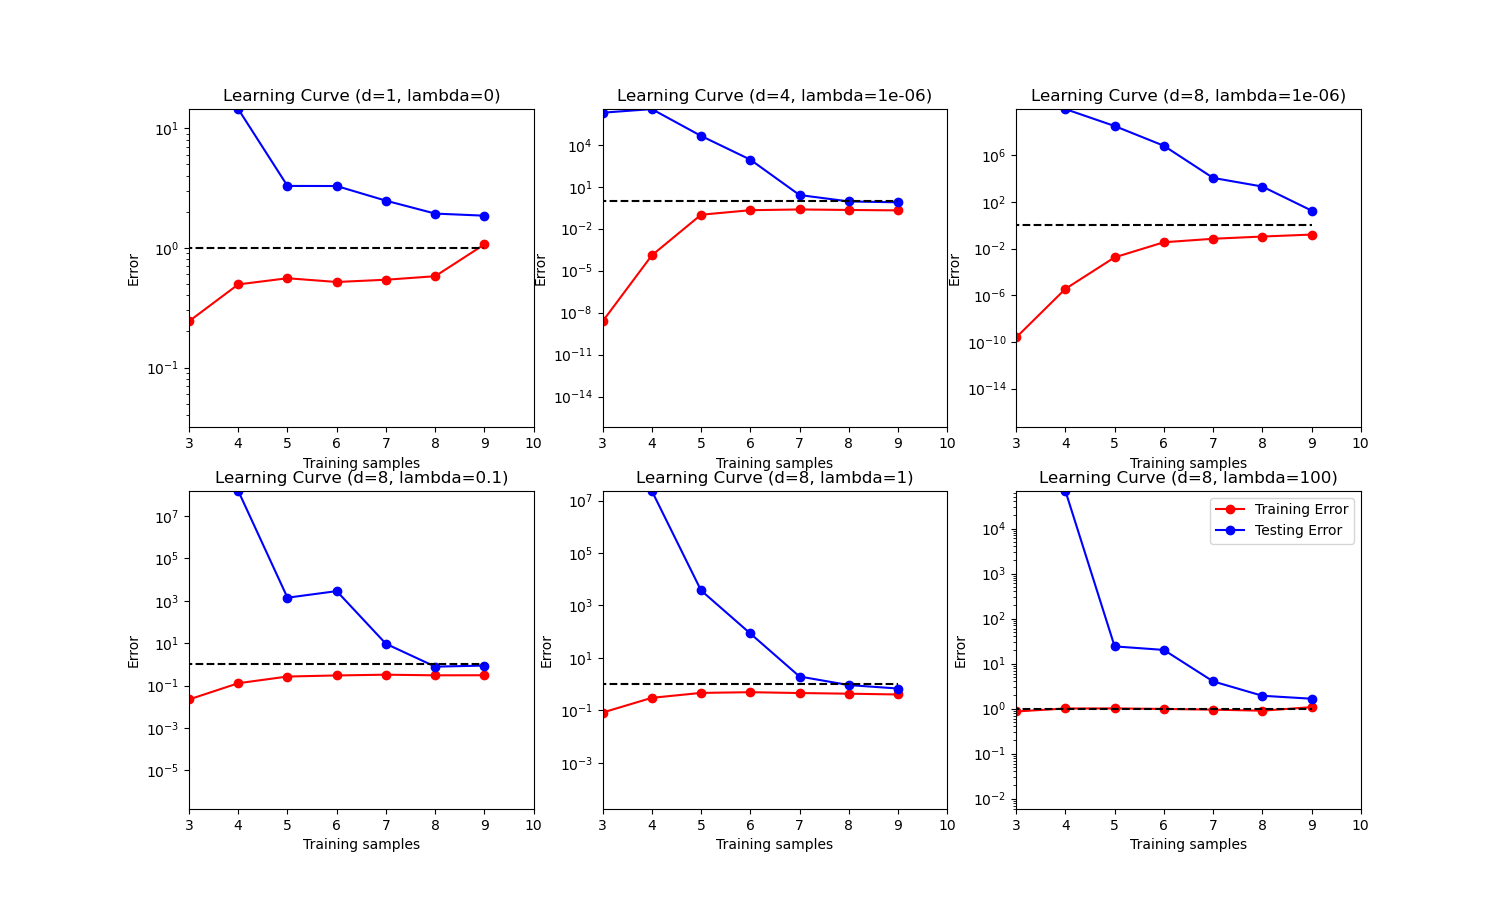
\includegraphics[width=0.9\textwidth]{/Users/ananyasoni/Desktop/cse/cse446/homework/hw1/learning_curves.png}
        \end{center}
    \end{tcolorbox}
\end{aprob}

\section*{Ridge Regression on MNIST}
\begin{aprob}
    In this problem we will implement a regularized least squares classifier for the MNIST data set. The task
    is to classify handwritten images of numbers between $0$ to $9$.\\
    
    You are \textbf{NOT} allowed to use any of the pre-built  classifiers in \verb|sklearn|.  Feel free to use any method from \verb|numpy| or \verb|scipy|. {\bf Remember:} if you are inverting a matrix in your code, you are probably doing something wrong (Hint: look at \verb|scipy.linalg.solve|).\\

    Each example has features $x_i \in \R^d$ (with $d=28*28=784$) and label $z_j \in \{0,\dots,9\}$. You can visualize a single example $x_i$ with \texttt{imshow} after reshaping it to its original $28 \times 28$ image shape (and noting that the label $z_j$ is accurate). We wish to learn a predictor $\widehat{f}$ that takes as input a vector in $\R^d$ and outputs an index in $\{0,\dots,9\}$. We define our training and testing classification error on a predictor $f$ as
    \begin{align*}
        \widehat{\epsilon}_{\textrm{train}}(f) &=
        \frac{1}{N _{\textrm{train}}} \sum_{(x,z)\in \textrm{Training Set}}     \1\{ f(x) \neq z \}
        \\
          \widehat{\epsilon}_{\textrm{test}}(f) &=
          \frac{1}{N _{\textrm{test}}} \sum_{(x,z)\in \textrm{Test Set}}     \1\{ f(x) \neq z \} 
    \end{align*}
    
    We will use one-hot encoding of the labels: for each observation $(x,z)$, the original label $z \in \{0, \ldots, 9\}$ is mapped to the standard basis vector $e_{z+1}$ where $e_i$ is a vector of size $k$ containing all zeros except for a $1$ in the $i^{\textrm{th}}$ position (positions in these vectors are indexed starting at one, hence the $z+1$ offset for the digit labels). We adopt the notation where we have $n$ data points in our training objective with features $x_i \in \R^d$ and label one-hot encoded as $y_i \in \{0,1\}^k$. Here, $k=10$ since there are 10 digits.
    
    \begin{enumerate}
        \item \points{10} In this problem we will choose a linear classifier to minimize the regularized least squares objective:
        \begin{align*}
            \widehat{W} = \text{argmin}_{W \in \R^{d \times k}} \sum_{i=1}^{n} \| W^Tx_{i} - y_{i} \|^{2}_{2} + \lambda \|W\|_{F}^{2}
        \end{align*}
        Note that $\|W\|_{F}$ corresponds to the Frobenius norm of $W$, i.e. $\|W\|_{F}^{2} = \sum_{i=1}^d \sum_{j=1}^k W_{i,j}^2$. To classify a point $x_i$ we will use the rule $\arg\max_{j=0,\dots,9} e_{j+1}^T \widehat{W}^T x_i$. Note that if $W = \begin{bmatrix} w_1 & \dots & w_k \end{bmatrix}$ then
        \begin{align*}
            \sum_{i=1}^{n} \| W^Tx_{i} - y_{i} \|^{2}_{2} + \lambda \|W\|_{F}^{2} &= \sum_{j=1}^k \left[  \sum_{i=1}^n ( e_j^T W^T x_i - e_j^T y_i)^2 + \lambda \| W e_j \|_2^2 \right] \\
            &= \sum_{j=1}^k \left[  \sum_{i=1}^n ( w_j^T x_i - e_j^T y_i)^2 + \lambda \| w_j \|_2^2 \right] \\
            &= \sum_{j=1}^k \left[  \| X w_j - Y e_j\|_2^2 + \lambda \| w_j \|_2^2 \right]
        \end{align*}
        where $X = \begin{bmatrix} x_1 & \dots & x_n \end{bmatrix}^\top \in \R^{n \times d}$ and $Y = \begin{bmatrix} y_1 & \dots & y_n \end{bmatrix}^\top \in \R^{n \times k}$. Show that
        \begin{align*}
            \widehat{W} = (X^T X + \lambda I)^{-1} X^T Y
        \end{align*} 

        \item \points{10} 
        \begin{itemize}
            \item Implement a function \verb|train| that takes as input $X \in\R^{n \times d}$, $Y \in \{0,1\}^{n \times k}$, $\lambda > 0$ and returns $\widehat{W} \in \R^{d \times k}$.
            \item Implement a function \verb|one_hot| that takes as input $Y \in \{0, ..., k-1\}^{n}$, and returns $Y \in \{0,1\}^{n \times k}$.
            \item Implement a function  \verb|predict| that takes as input $W \in \R^{d \times k}$, $X' \in\R^{m \times d}$ and returns an $m$-length vector with the $i$th entry equal to $\arg\max_{j=0,\dots,9} e_j^T W^T x_i'$ where $x_i' \in \R^d$ is a column vector representing the $i$th example from $X'$.
            \item Using the functions you coded above, train a model to estimate $\widehat{W}$ on the MNIST training data with $\lambda = 10^{-4}$, and make label predictions on the test data. This behavior is implemented in \verb|main| function provided in zip file. {\bf What is the training and testing error?} Note that they should both be about $15\%$. 
        \end{itemize}
    \end{enumerate}
    
    \subsubsection*{What to Submit:}
    \begin{itemize}
        \item \textbf{Part A:} Derivation of expression for $\widehat{W}$
        \item \textbf{Part B:} Values of training and testing errors
        \item \textbf{Code} on Gradescope through coding submission
    \end{itemize}
    \begin{tcolorbox}[colback=lightgray!10!white, colframe=black, title=A5.a, breakable]
        \begin{center}
            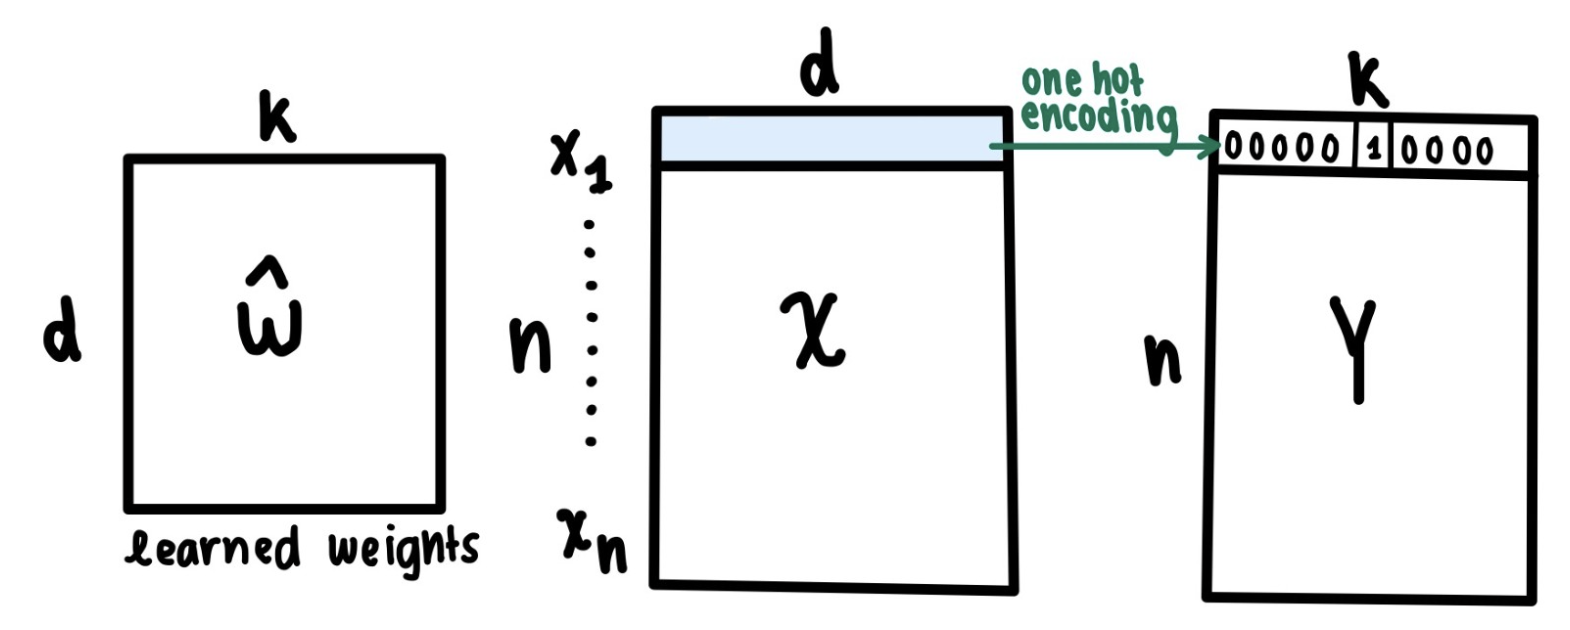
\includegraphics[width=0.8\textwidth]{A5dimensions.png}
        \end{center}
        
        We want to show that $\widehat{W} = (X^T X + \lambda I)^{-1} X^T Y$ minimizes the regularized least squares objective.
        
        Given the objective function:
        \begin{align*}
        \widehat{W} &= \text{argmin}_{W \in \mathbb{R}^{d \times k}} \sum_{i=1}^{n} \| W^Tx_{i} - y_{i} \|^{2}_{2} + \lambda \|W\|_{F}^{2}\\
        &= \text{argmin}_{W \in \mathbb{R}^{d \times k}} \sum_{j=1}^k \left[ \| X w_j - Y e_j\|_2^2 + \lambda \| w_j \|_2^2 \right]
        \end{align*}
        
        We can minimize each term in the sum independently. For each $j \in \{1, 2, \ldots, k\}$. Since the regularized loss decomposes into a sum over each $j$, we can minimize each $f(w_j)$ independently.
        We need to minimize:
        \begin{align*}
        f(w_j) = \| X w_j - Y e_j\|_2^2 + \lambda \| w_j \|_2^2
        \end{align*}
        
        We can expand the expression using the property that $\|x\|_2^2 = x^T x$ from the linear algebra review guide:
        \begin{align*}
        % f(w_j) &= (X w_j - Y e_j)^T (X w_j - Y e_j) + \lambda w_j^T w_j\\
        % &= w_j^T X^T X w_j - w_j^T X^T Y e_j - e_j^T Y^T X w_j + e_j^T Y^T Y e_j + \lambda w_j^T w_j
        f(w_j) &= \|X w_j - Y e_j\|_2^2 + \lambda \|w_j\|_2^2 & \text{(original objective)} \\
        &= (X w_j - Y e_j)^T (X w_j - Y e_j) + \lambda w_j^T w_j & \text{(using $\|x\|_2^2 = x^T x$)} \\
        &= (w_j^T X^T - e_j^T Y^T)(X w_j - Y e_j) + \lambda w_j^T w_j & \text{(matrix transpose property)} \\
        &= w_j^T X^T X w_j - w_j^T X^T Y e_j - e_j^T Y^T X w_j + e_j^T Y^T Y e_j + \lambda w_j^T w_j & \text{(distributive property)}
        \end{align*}
        
        Since $e_j^T Y^T X w_j$ is a scalar, it equals its transpose $w_j^T X^T Y e_j$, so:
        \begin{align*}
        % f(w_j) &= w_j^T X^T X w_j - 2e_j^T Y^T X w_j + e_j^T Y^T Y e_j + \lambda w_j^T w_j\\
        % &= w_j^T(X^T X + \lambda I)w_j - 2e_j^T Y^T X w_j + e_j^T Y^T Y e_j
        f(w_j) &= w_j^T X^T X w_j - w_j^T X^T Y e_j - e_j^T Y^T X w_j + e_j^T Y^T Y e_j + \lambda w_j^T w_j \\
        &= w_j^T X^T X w_j - 2e_j^T Y^T X w_j + e_j^T Y^T Y e_j + \lambda w_j^T w_j & \text{(since $e_j^T Y^T X w_j = w_j^T X^T Y e_j$)} \\
        &= w_j^T(X^T X)w_j - 2e_j^T Y^T X w_j + e_j^T Y^T Y e_j + \lambda w_j^T w_j & \text{(associative property)} \\
        &= w_j^T(X^T X)w_j + \lambda w_j^T w_j - 2e_j^T Y^T X w_j + e_j^T Y^T Y e_j & \text{(rearranging terms)} \\
        &= w_j^T(X^T X + \lambda I)w_j - 2e_j^T Y^T X w_j + e_j^T Y^T Y e_j & \text{(factoring out $w_j^T$ and $w_j$)}
        \end{align*}
        
        % To find the minimum, we compute the gradient with respect to $w_j$ and set it to zero:
        % \begin{align*}
        % \nabla_{w_j} f(w_j) &= 2(X^T X + \lambda I)w_j - 2X^T Y e_j = 0\\
        % \Rightarrow (X^T X + \lambda I)w_j &= X^T Y e_j\\
        % \Rightarrow w_j &= (X^T X + \lambda I)^{-1} X^T Y e_j
        % \end{align*}
        To find the minimum, we compute the gradient with respect to $w_j$ and set it to zero.
        \begin{align*}
        \nabla_{w_j} f(w_j) &= \nabla_{w_j}[w_j^T(X^T X + \lambda I)w_j - 2e_j^T Y^T X w_j + e_j^T Y^T Y e_j] \\
        &= \nabla_{w_j}[w_j^T(X^T X + \lambda I)w_j] - \nabla_{w_j}[2e_j^T Y^T X w_j] + \nabla_{w_j}[e_j^T Y^T Y e_j] \\
        \end{align*}
        
        For the first term, we use the property that $\nabla_x(x^TAx) = 2Ax$ for symmetric matrices $A$. Note that $(X^T X + \lambda I)$ is symmetric:
        \begin{align*}
        \nabla_{w_j}[w_j^T(X^T X + \lambda I)w_j] &= 2(X^T X + \lambda I)w_j & \text{(quadratic form derivative)}
        \end{align*}
        
        For the second term, we use the property that $\nabla_x(b^Tx) = b$ for any constant vector $b$:
        \begin{align*}
        \nabla_{w_j}[2e_j^T Y^T X w_j] &= 2X^T Y e_j & \text{(note: $b = 2X^T Y e_j$)}
        \end{align*}
        
        For the third term, since $e_j^T Y^T Y e_j$ doesn't contain $w_j$, its derivative is zero:
        \begin{align*}
        \nabla_{w_j}[e_j^T Y^T Y e_j] &= 0
        \end{align*}
        
        Combining these terms:
        \begin{align*}
        \nabla_{w_j} f(w_j) &= 2(X^T X + \lambda I)w_j - 2X^T Y e_j + 0 \\
        &= 2(X^T X + \lambda I)w_j - 2X^T Y e_j
        \end{align*}
        
        Setting equal to zero we get the following:
        \begin{align*}
        2(X^T X + \lambda I)w_j - 2X^T Y e_j &= 0 \\
        \Rightarrow (X^T X + \lambda I)w_j &= X^T Y e_j \\
        \Rightarrow w_j &= (X^T X + \lambda I)^{-1} X^T Y e_j
        \end{align*}
         
        Since $Y e_j$ is the $j$-th column of $Y$, and this solution holds for all $j \in \{1, 2, \ldots, k\}$, we can write:
        \begin{align*}
        W = [w_1, w_2, \ldots, w_k] = (X^T X + \lambda I)^{-1} X^T Y
        \end{align*}
        
        Therefore:
        \begin{align*}
        \widehat{W} = (X^T X + \lambda I)^{-1} X^T Y
        \end{align*}
        
        This is guarenteed to be the global minimum because the Hessian of $f(w_j)$ is $2(X^T X + \lambda I)$, which is positive definite because $X^T X$ is positive semidefinite and $\lambda > 0$. \\
        \end{tcolorbox}
        \begin{tcolorbox}[colback=lightgray!10!white, colframe=black, title=A5.b, breakable]
            \textbf{Training Error:} 14.805\% \\
            \textbf{Testing Error:} 14.66\%
        \end{tcolorbox}
\end{aprob}

\end{document}

%%% Local Variables:
%%% mode: latex
%%% TeX-master: t
%%% End:
